\documentclass[border=6.5pt]{standalone}

\usepackage[utf8]{inputenc}
\usepackage{garamondx}

\usepackage[x11names]{xcolor}

\definecolor{darkolivegreen}{rgb}{0.33, 0.42, 0.18}
\definecolor{darkbyzantium}{rgb}{0.36, 0.22, 0.33}
\definecolor{darkelectricblue}{rgb}{0.33, 0.41, 0.47}
\definecolor{deepchestnut}{rgb}{0.73, 0.31, 0.28}

\usepackage{tikz}
\usetikzlibrary{shapes.geometric, positioning, calc, arrows, decorations.markings}

\tikzstyle{background}=[rectangle, rounded corners, minimum width=7em, minimum height=2em, text centered, draw=black, fill=darkolivegreen!30, text width=7em]
\tikzstyle{process} = [rectangle, rounded corners, minimum width=7em, minimum height=2em, text centered, draw=black, fill=darkbyzantium!30, text width=7em]
\tikzstyle{psych}=[rectangle, rounded corners, minimum width=7em, minimum height=2em, text centered, draw=black, fill=darkelectricblue!30, text width=7em]
\tikzstyle{local}=[rectangle, rounded corners, minimum width=7em, text centered, draw=black, fill=deepchestnut!30, text width=7em]
\tikzstyle{arrow}=[very thick, <->, >=latex]

\begin{document}

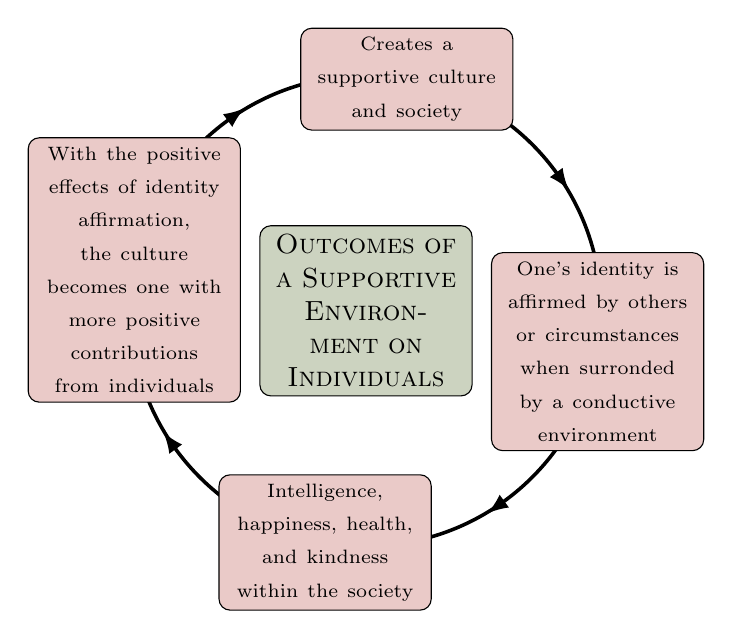
\begin{tikzpicture}[decoration = {markings,
    mark = between positions 0.1 and 1 step 0.25 with {\arrow[>=latex, ultra thick]{<}}}]
	\def \radius {8.5em}
	
  		\draw[postaction = decorate, line width=0.3ex] (0, 0) circle [radius=\radius];
  		\path (80 :\radius) node[local]{\scriptsize Creates a supportive culture and society}
        (350:\radius) node[local]{\scriptsize One's identity is affirmed by others or circumstances when surronded by a conductive environment}
        (260:\radius) node[local]{\scriptsize Intelligence, happiness, health, and kindness within the society}
        (170:\radius)node[local]{\scriptsize With the positive effects of identity affirmation, the culture becomes one with more positive contributions from individuals};
        \node[background]{\textsc{Outcomes of a Supportive Environment on Individuals}};
\end{tikzpicture}

\end{document}
